\documentclass{beamer}

\usepackage[utf8]{inputenc}
\usepackage[T1]{fontenc}
\usepackage{setspace}
\usepackage{color}
\usepackage{listings}
\usepackage{hyperref}
\usepackage{graphicx}

\usepackage[scaled]{beramono}
\newcommand\Small{\fontsize{9}{9.2}\selectfont}
\newcommand\LSTfont{\Small\ttfamily}

\usetheme{Dresden}

\title{i18n \& l10n: Internationalization and Localization in Rails}
\author{Constantin Hofstetter}
\date{\today}

\begin{document}

\lstset{ %
language=Ruby,                % choose the language of the code
basicstyle=\LSTfont,       % the size of the fonts that are used for the code
stepnumber=1,                   % the step between two line-numbers. If it is 1 each line will be numbered
numbersep=5pt,                  % how far the line-numbers are from the code
backgroundcolor=\color{white},  % choose the background color. You must add \usepackage{color}
showspaces=false,               % show spaces adding particular underscores
showstringspaces=false,         % underline spaces within strings
showtabs=false,                 % show tabs within strings adding particular underscores
frame=false,           % adds a frame around the code
tabsize=2,          % sets default tabsize to 2 spaces
captionpos=b,           % sets the caption-position to bottom
breaklines=true,        % sets automatic line breaking
breakatwhitespace=false,    % sets if automatic breaks should only happen at whitespace
escapeinside={\%*}{*)},          % if you want to add a comment within your code
keywordstyle=\color{blue},
stringstyle=\color{red},
commentstyle=\color{green},
morecomment=[l][\color{magenta}]{\#}
}

\begin{frame}
\titlepage
\end{frame}

\begin{frame}
\frametitle{Definitions}
\begin{block}{i18n - Internationalization}
Design the application so that it can potentially be adapted to various languages and regions (\lstinline{i18n} gem is part of Rails)
\end{block}
\begin{block}{l10n - Localization}
The process of adapting internationalized software for a specific region or language by adding locale-specific components and translating text
\end{block}
\end{frame}

\begin{frame}[fragile]{Preparations}
\begin{block}{Raise an exception on missing translations}
\begin{lstlisting}
# config/environments/test.rb
# and
# config/environments/development.rb
Rails.application.configure do |config|
  config.action_view.raise_on_missing_translations = true
end
\end{lstlisting}
\end{block}
\begin{block}{Instead of \lstinline{I18n.t()} use \lstinline{t()} shortcut in tests}
\begin{lstlisting}
RSpec.configure do |config|
  config.include AbstractController::Translation
end
\end{lstlisting}
\Small{See "\href{http://robots.thoughtbot.com/foolproof-i18n-setup-in-rails}{Foolproof i18n setup on Thoughtbot}"}
\end{block}
\end{frame}

\begin{frame}[fragile]{Best practices: Design}

\begin{block}{Make sure things look pretty with a different text length}

Other locales will have longer (or shorter) texts: make sure things still look fine.

\end{block}

\begin{block}{Internationalize user interface}

Remember that some locales might require text from right to left (e.g. arabic). Also check for user input (e.g. a SlimWiki user from Saudi Arabia).

\end{block}

\end{frame}


\begin{frame}[fragile]{Best practices}

\begin{block}{Use correct ISO code for locale}

Adapt for different regions: e.g. en-US (American English: color) vs. en-UK (British English: colour)

\Small{See \href{https://github.com/tigrish/iso}{https://github.com/tigrish/iso} for a comprehensive list}

\end{block}

\end{frame}

\begin{frame}[fragile]{Pluralization}

\begin{block}{Rules}

Either add your own \lstinline{config/plurals.rb} or add \lstinline{gem 'rails-18n'} to your GEMFILE.

\end{block}

\begin{block}{Localization}
\begin{lstlisting}
# de:
#   plurals:
#     elephant:
#       zero: 'Elefant'
#       one: 'Elefant'
#       other: 'Elefanten'

I18n.locale = :de
I18n.t('plurals.elephant', count: 2) => Elefanten
\end{lstlisting}
\end{block}


\end{frame}

\begin{frame}[fragile]{Interpolation}

\begin{block}{Example}
\begin{lstlisting}
#
# en:
#   hello_user: "Hello %{ name }"
#

I18n.locale = :en
I18n.t('hello_user', name: 'Constantin') => "Hello Constantin"
\end{lstlisting}
\end{block}
\end{frame}

\begin{frame}[fragile]{i18n: Front end}
\begin{block}{Regular views}

Use the \href{https://github.com/douglasjsellers/herbgobbler}{\lstinline{HerbGobbler}} gem to add all your plaintext to a yml.

You will still need to manually go through all files to add missing strings (e.g. obscure html) and fix interpolations.

\end{block}

\begin{block}{Static javascript}

Add the \href{https://github.com/fnando/i18n-js}{\lstinline{i18n-js}} gem for translation helpers in javascript.

Create a custom js file to minimize file size.

\end{block}
\end{frame}


\begin{frame}[fragile]{i18n: Database}
\begin{block}{ActiveRecord models}

Use the \href{https://github.com/globalize/globalize}{\lstinline{Globalize}} gem to translate ActiveRecord model attributes.

\begin{lstlisting}
  # The model
  class Post < ActiveRecord::Base
    translates :title, :text
  end

  # The migration
  class AddTranslationsToPosts < ActiveRecord::Migration
    def up
      Post.create_translation_table! :title => :string, :text => :text
    end
    def down
      Post.drop_translation_table!
    end
  end
\end{lstlisting}

\end{block}
\end{frame}

\begin{frame}[fragile]{Tools}
\begin{block}{i18n-tasks}

The \href{https://github.com/globalize/globalize}{\lstinline{i18n-tasks}} gem helps you find and manage missing and unused translations.

\begin{figure}[ht!]
\centering
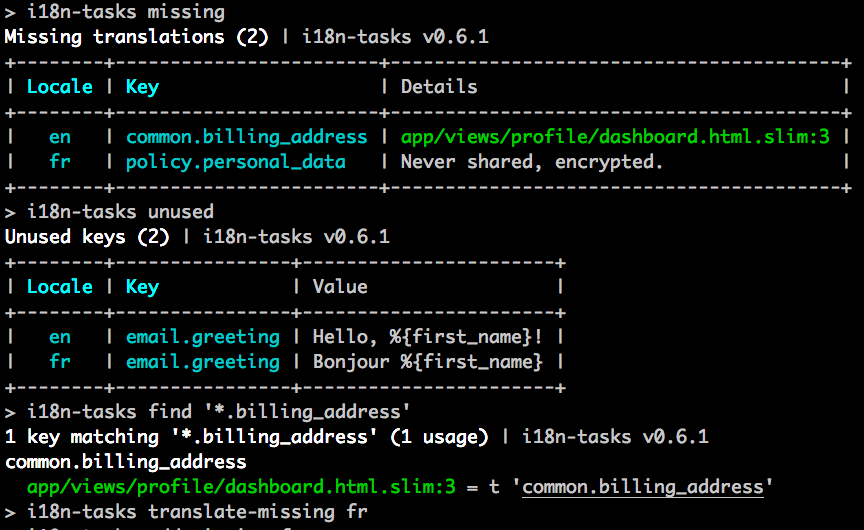
\includegraphics[width=77mm]{i18ntasks.png}
\end{figure}

\end{block}
\end{frame}

\begin{frame}[fragile]{l10n: Translating the strings}
\begin{block}{Use a webservice}

Use a webservice such as \href{http://localeapp.com}{LocaleApp} or \href{http://webtranslateit.com}{WebTranslateIt} to get files translated.

\end{block}

\begin{block}{Start early}
Start the translation process early - you can work on preparing the frontend and application logic while the files get translated.
\end{block}

\end{frame}

\begin{frame}[fragile]{Application Logic}
\begin{block}{use a \lstinline{before_action}}

\begin{lstlisting}
  # in ApplicationController
  before_action :set_locale

  def set_locale
    I18n.locale = case request.host
                  when  /[\da-z\.-]*\.co\.uk$/
                    "en-UK"
                  else
                    "en-US"
                  end
  end
\end{lstlisting}

\end{block}

\begin{block}{Store prefered locale in User model}
If a user chooses a locale, make sure to save it in the database.
\end{block}

\end{frame}

\begin{frame}[fragile]{SEO gotchas}

\begin{block}{SEO?}
Search Engine Optimization: How not to get penalized by Google.
\end{block}

\end{frame}


\begin{frame}[fragile]{SEO}

\begin{block}{How to determine the locale?}
\begin{itemize}
\item by tld e.g. \lstinline{.fr, .de} (good!)

\item by path \lstinline{.com/de, .com/fr} (ok!)

\item by parameter \lstinline{.com/?ln=de} or cookie (bad!)
\end{itemize}

\end{block}

\begin{block}{What to do with duplicate content?}
\begin{itemize}
\item block with robots.txt (not that good)
\item redirect and/or set canonical url (better)
\end{itemize}

\Small{See \href{https://support.google.com/webmasters/answer/182192}{https://support.google.com/webmasters/answer/182192}}
\end{block}

\end{frame}

\begin{frame}[fragile]{SEO}

\begin{block}{Sitemap}
Use a sitemap to indicate same site is available in different language (resource has to include itself)
\begin{lstlisting}
  <url>
    <loc>http://oozou.com</loc>
    <xhtml:link
                 rel="alternate"
                 hreflang="de"
                 href="http://oozou.de"
                 />
    <xhtml:link
                 rel="alternate"
                 hreflang="en"
                 href="http://oozou.com"
                 />
  </url>
\end{lstlisting}
\Small{See \href{https://support.google.com/webmasters/answer/2620865}{https://support.google.com/webmasters/answer/2620865}}

\end{block}

\end{frame}

\begin{frame}[fragile]{SEO}

\begin{block}{hreflang link tags}
Use hreflang for language and regional URLs (resource has to include itself)
\begin{lstlisting}
<head>
<link rel="alternate" href="http://oozou.com" hreflang="en" />
<link rel="alternate" href="http://oozou.th"  hreflang="th" />
<link rel="alternate" href="http://oozou.de"  hreflang="de" />
<link rel="alternate" href="http://oozou.jp"  hreflang="jp" />
</head>
\end{lstlisting}
\Small{See \href{https://support.google.com/webmasters/answer/189077}{https://support.google.com/webmasters/answer/189077}}

\end{block}

\end{frame}

\begin{frame}[fragile]{SEO}

\begin{block}{Target countries with different TLDs}
Use Google Webmaster tools to target different countries based on your domain.

This only works with gTLDs (generic top-level domain names: e.g. \lstinline{.com, .net}) and not with ccTLDs (country-code top-level domain names: e.g. \lstinline{.de, .th}).

\Small{See \href{https://support.google.com/webmasters/answer/1347922}{https://support.google.com/webmasters/answer/1347922}}

\end{block}

\begin{block}{Analytics}
Make sure to track traffic changes in analytics based on countries and locales. Adjust country targeting appropriately.
\end{block}


\end{frame}

\end{document}
